\appendix
\addcontentsline{toc}{part}{Annexes}
\chapter{Organisation du projet PIGA-SYSTRANS}
	\label{PIGA_SYSTRANS tech}
	
	\paragraph*{}
		Le projet PIGA-SYSTRANS est constitué de 3 parties:
		\begin{itemize}
   			\item Contextd: C'est le cœur du système. Le daemon va analyser les états internes des programmes et effectuer les actions décrites dans ses fichiers de règles;
   			\item LibContext: Bibliothèque en C permettant de faciliter l'envoi de l'état interne d'un programme;
   			\item Context-Notify: Propose une interface graphique d'interaction avec Contextd.
   		\end{itemize}
		
	\paragraph*{}
		Mon travail a consisté en l'écriture de contextd, libcontext et de la formalisation de l'écriture de règles de sécurité en XML. Le travail a ensuite consisté en la création de plugins pour Firefox et Claws-mail avec éventuellement un peu de patchage (pour claws-mail notamment).	
		
	\paragraph*{}
		Ce projet, représentant environ 5000 lignes de code, a majoritairement été écrit en C/C++ et le framework Qt. On y trouve cependant aussi du XUL/Javascript et du C/GTK pour respectivement les plugins Firefox et Claws-mail.


	\paragraph*{}
		Pour un schéma des interactions, veuillez vous reporter à la figure \ref{schema_piga_systrans}.
	
	\section{Contextd}
		\paragraph*{}
			Contextd a une architecture orientée plugin. Ceux-ci sont liés statiquement et sont désactivables un à un par l'utilisation de defines à la compilation. Ces plugins permettent une meilleure séparation du code ce qui simplifie donc la maintenance et les potentiels effets de bord. De plus, le daemon est donc devenu event-driven.
		
		\paragraph*{}	
			Son cœur est composé de 3 fonctions majeures:
			\begin{itemize}
   				\item La daemonisation: Le programme doit se daemoniser au démarrage pour tourner en tâche de fond.
   				\item L'écoute et l'émission d'appels et signaux D-Bus sur le bus système com.piga.contextd.
   				\item L'interprétation des règles et leur mise en correspondance avec les données utilisateur.
   			\end{itemize}
   			
   		\paragraph*{}
   			Une fois la mise en correspondance des données utilisateurs effectuée, des événements sont envoyés et broadcastés à tous les plugins. Pour plus d'informations sur les événements envoyés, vous pouvez vous reporter au dossier \emph{srccontextd/src/plugins}.
   			
   		\paragraph*{}
   			Voici la liste des différents plugins:
   			\begin{itemize}
   				\item iptables-blocker: Ajoute/enlève dynamiquement des règles dans le pare-feu iptables de façon à laisser un programme accéder à un site pour lequel contextd a validé l'accès.
   				\item killer: Envoi un signal (généralement un SIG\_KILL) à un programme lorsqu'il rentre dans un état que l'on considère invalide.
   				\item logger: Loggue tout les événements dans syslog-ng.
   				\item notify: Affiche à l'écran des notifications qu'il juge importante en utilisant libnotify.
   				\item selinux: Charge des modules SELinux dynamiquement par application en fonction du contexte global.
   			\end{itemize}
   			   			
   		\paragraph*{}
   			L'écriture des règles est détaillé à l'annexe \ref{PIGA_SYSTRANS TRAC} mais aussi à l'adresse \emph{https://www.sds-project.fr/trac/PIGA-SYSTRANS/wiki/doc\_contextd}.
   					
	\section{libcontext}
		\paragraph*{}
			Libcontext facilite la communication entre les applications et contextd. La communication utilise l'IPC D-Bus. Libcontext se connecte sur le bus system com.piga.contextd et a ensuite accès aux différentes méthodes exportées par le daemon.
			
		\paragraph*{}
			Pour envoyer son état interne, il faut en premier s'enregistrer sur le daemon puis ensuite appeler une fonction à paramètres infinie. Ces paramètres permettent de définir des couples "nom/valeur". La liste se termine par le couple "NULL/NULL".\\
			Si vous cherchez un exemple d'utilisation, vous pouvez regarder le fichier \emph{plugins/claws\-mail/piga\_context/src/piga\_context.c}.
			
		\paragraph*{}
			Pour utiliser libcontext, vous devez en premier linker avec. Pour ce faire, vous pouvez utiliser pkgconfig qui vous donnera les flags à ajouter à gcc : \emph{pkg-config --cflags --libs context}.
			
		\paragraph*{}
			Pour plus de détails sur l'API, veuillez consulter l'annexe \ref{PIGA_SYSTRANS Libcontext Interface}.
		
	\section{Context-notify}
		\paragraph*{}
			Context-notify permet d'apporter une plus grande interaction entre l'utilisateur et le daemon.
			
		\paragraph*{}
			Il est composé de deux parties:
			\begin{itemize}
   				\item La fenêtre de changement manuel de context (voir figure \ref{context-notify change context});
   				\item La popup de demande d'autorisation de transition de context (voir figure \ref{context-notify autorisation}).
   			\end{itemize}
			
		\begin{figure}[!h]
			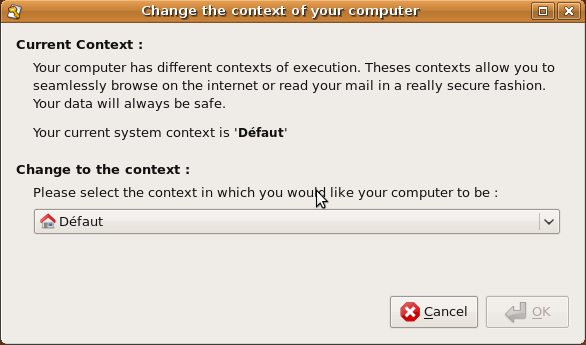
\includegraphics[width=11cm]{images/contextnotifydlg.png}
			\caption{Fenêtre de changement manuel de contexte}
			\label{context-notify change context}
		\end{figure}
		
		\begin{figure}[!h]
			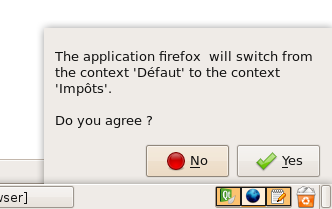
\includegraphics[width=7cm]{images/contextnotifypopup.png}
			\caption{Demande d'autorisation de transition}
			\label{context-notify autorisation}
		\end{figure}

	%Figure qui montre tout le userspace
	\begin{figure}[!h]
		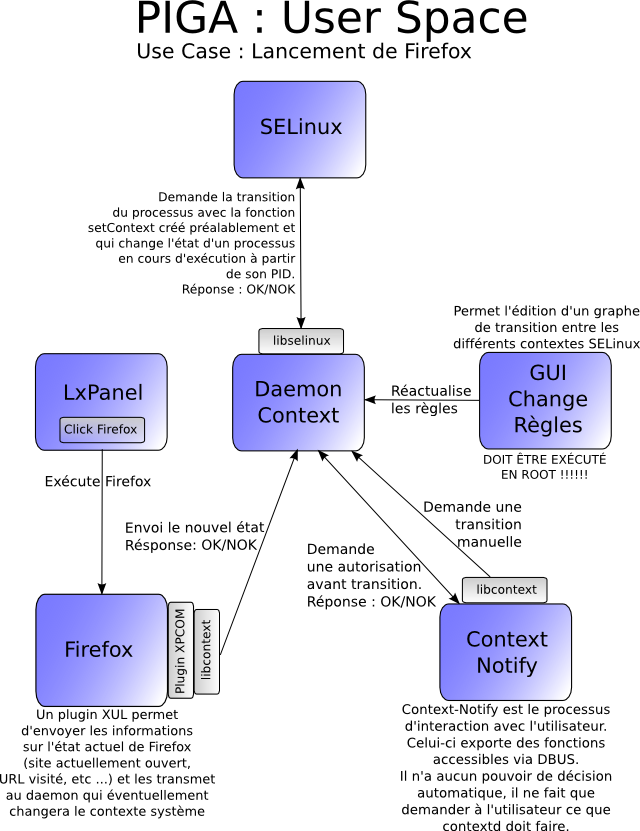
\includegraphics[width=17cm]{images/userspace.png}
		\caption{Schéma des interactions dans PIGA-SYSTRANS}
		\label{schema_piga_systrans}
	\end{figure}
		
\chapter{Les plugins}
	\label{PIGA_SYSTRANS plugins}
	
	\paragraph*{}
		Pour l'intégration de PIGA-SYSTRANS dans les applications, l'utilisation de plugins a semblé la meilleure option car elle est la plus pérenne/demande peu de temps à maintenir.
		
	\paragraph*{}
		Chaque plugin réalise deux tâches essentielles:
		\begin{itemize}
   			\item Transmettre l'état actuel du programme;
   			\item Changer dynamiquement l'affichage en fonction du contexte actuel et de ses droits;
   		\end{itemize}
	
	\section{Firefox}
		\paragraph*{}
			Le plugin Firefox réalise les deux tâches essentielles mais il se charge aussi de vider le cache lors d'un changement de contexte.
			
		\paragraph*{}
			Il est composé de deux parties:
			\begin{itemize}
   				\item Un plugin binaire XPCOM, écrit en C. Il permet d'établir le dialogue avec le daemon;
   				\item Un plugin Javascript. Il se charge de récupérer les événements utilisateur, de modifier l'interface graphique et de vider le cache lors des changements de contexte.
   			\end{itemize}
   			
   		\begin{figure}[!h]
			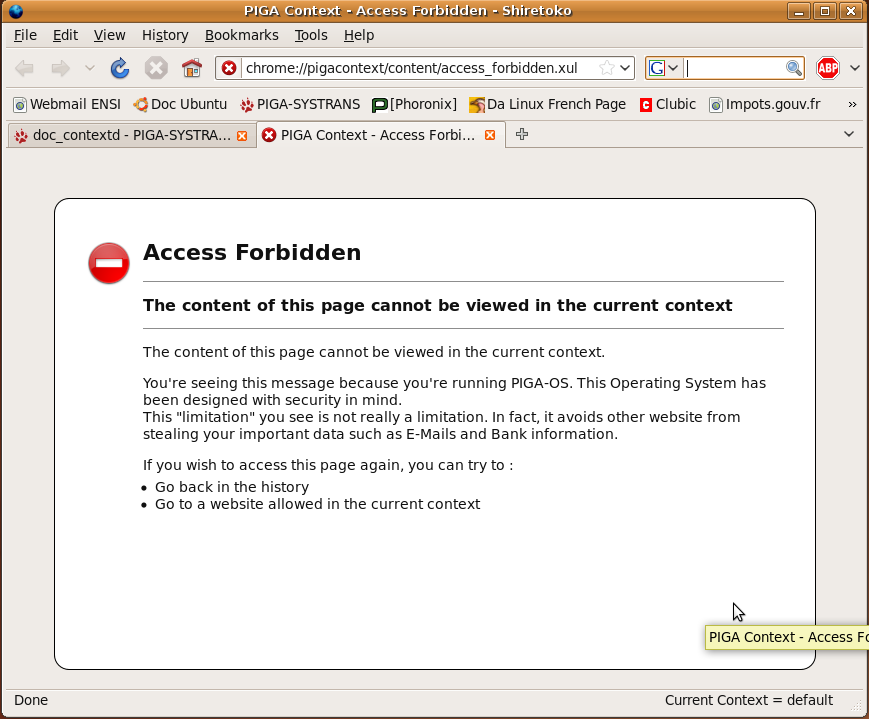
\includegraphics[width=13cm]{images/firefox.png}
			\caption{Exemple d'une modification faite à Firefox}
		\end{figure}
	
	\section{Claws-mail}
		\paragraph*{}
			Le plugin Claws-mail a été écrit en C/GTK. Cependant, contrairement à Firefox, il a nécessité des modifications dans le code de Claws-mail.
			
		\paragraph*{}
			En effet, Claws-mail n'avait aucun hook lors de l'ouverture d'un email et manquait aussi d'un système d'affichage d'erreur personnalisé à la place d'un email. Cela a été ma première tâche.
			
		\paragraph*{}
			Ces modifications ont été faites avec l'aval de l'équipe de Claws-mail. Pour ce faire, j'ai travaillé avec eux via IRC en leur expliquant premièrement ce que j'allais faire puis en leur soumettant des versions de test pour qu'ils puissent les pré-valider.\\
			Ce travail a été très intéressant et a été l'occasion de produire mon premier patch pour un programme autre que le mien. Je voudrais aussi saluer le professionnalisme de l'équipe, pourtant petite, qui montre bien que le logiciel libre n'est pas du travail d'amateur.
			
		\paragraph*{}
			Le patch final, qui fait environ 200 lignes, se trouve à l'adresse \emph{plugins/claws\-mail/mail\_pre\_open\_hook.patch}. Il sera proposé à la communauté pour approbation finale quand il aura été validé de notre coté.
			
		\begin{figure}[!h]
			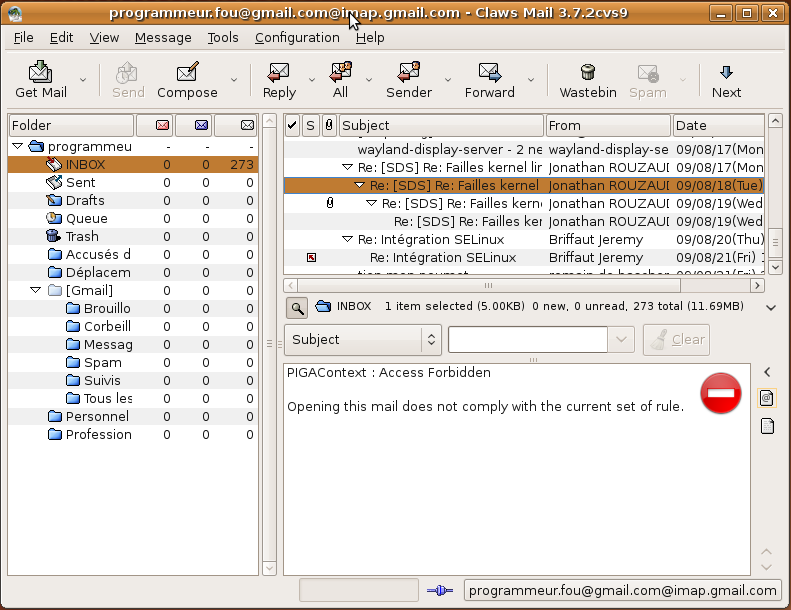
\includegraphics[width=13cm]{images/clawsmail.png}
			\caption{Exemple d'une modification faite à Claws-mail}
		\end{figure}
	
	\section{Open Office}
		\paragraph*{}
			Je n'ai malheureusement pas eu le temps d'aller plus loin que la recherche d'informations sur les plugins UNO.
			
		\paragraph*{}
			Ce plugin n'a donc pas pu être développé.
	
\chapter{Libcontext's Interface}
	\label{PIGA_SYSTRANS Libcontext Interface}
	{\tt \#include $<$string.h$>$}\par


Include dependency graph for libcontext.h:\nopagebreak
\begin{figure}[H]
\begin{center}
\leavevmode
\begin{figure}[!h]
	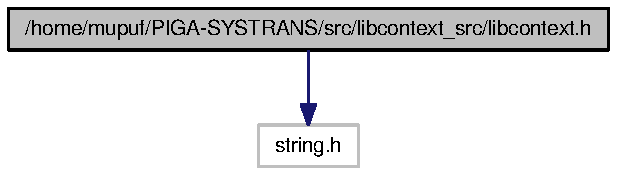
\includegraphics[width=166pt]{doxygen/libcontext_8h__incl}
	\caption{libcontext.h's dependency graph}
\end{figure}
\end{center}
\end{figure}


This graph shows which files directly or indirectly include this file:\nopagebreak
\begin{figure}[H]
\begin{center}
\leavevmode
\begin{figure}[!h]
	\includegraphics[width=357pt]{doxygen/libcontext_8h__dep__incl}
	\caption{libcontext.h is a dependency of ...}
\end{figure}
\end{center}
\end{figure}
\subsection*{Typedefs}
\begin{CompactItemize}
\item 
typedef void($\ast$ {\bf contextChangedCallbackSuccess} )(unsigned int id, {\bf context\_\-result} result)\label{libcontext_8h_5dda83b6631815ae03c1e487a549ba4a}

\begin{CompactList}\small\item\em id= \item\end{CompactList}\item 
typedef void($\ast$ \textbf{contextChangedCallbackError} )(unsigned int id, const char $\ast$error, const char $\ast$message)\label{libcontext_8h_5565e3ea8ade2cb600ae3b07aca2c281}

\item 
typedef void($\ast$ \textbf{contextChangedCallback} )(const char $\ast$previousContext, const char $\ast$nextContext, void $\ast$user\_\-data)\label{libcontext_8h_2fe3b642ce5c55f396c7889da7365fa3}

\end{CompactItemize}
\subsection*{Enumerations}
\begin{CompactItemize}
\item 
enum {\bf context\_\-bool} \{ {\bf CONTEXT\_\-FALSE} = 0, 
{\bf CONTEXT\_\-TRUE} = 1
 \}
\begin{CompactList}\small\item\em Define a boolean. \item\end{CompactList}\item 
enum {\bf context\_\-result} \{ {\bf CONTEXT\_\-ACCEPTED} = 0, 
{\bf CONTEXT\_\-REFUSED} = 1, 
{\bf CONTEXT\_\-ERROR} = 2
 \}
\begin{CompactList}\small\item\em Define context\_\-result. \item\end{CompactList}\end{CompactItemize}
\subsection*{Functions}
\begin{CompactItemize}
\item 
{\bf context\_\-bool} {\bf context\_\-is\_\-registered} ()
\begin{CompactList}\small\item\em Is your application already registered ? \item\end{CompactList}\item 
{\bf context\_\-bool} {\bf context\_\-register\_\-application} (const char $\ast$app\_\-name)
\begin{CompactList}\small\item\em Register your application onto the context Daemon. \item\end{CompactList}\item 
{\bf context\_\-result} {\bf context\_\-changed} (const char $\ast$param\_\-name,...)
\begin{CompactList}\small\item\em Send your internal context to the daemon. Should be called like this: context\_\-changed(var1\_\-name, var1\_\-data, var2\_\-name, var2\_\-data, ..., NULL, NULL);. \item\end{CompactList}\item 
unsigned int {\bf context\_\-changed\_\-async} ({\bf contextChangedCallbackSuccess} success\_\-cb, contextChangedCallbackError error\_\-cb, const char $\ast$param\_\-name,...)
\begin{CompactList}\small\item\em It the same than context\_\-changed but async, see \doxyref{context\_\-changed()}{p.}{libcontext_8h_efe26a27281f13bf1a919ca652c93f3c} for more details. \item\end{CompactList}\item 
{\bf context\_\-bool} {\bf context\_\-required\_\-context} (char $\ast$required\_\-context, size\_\-t maxlen, const char $\ast$param\_\-name,...)
\begin{CompactList}\small\item\em Checks what would be the system context if we had sent this state to the daemon. This is the same logic than \doxyref{context\_\-changed()}{p.}{libcontext_8h_efe26a27281f13bf1a919ca652c93f3c} with only some extra parameters. \item\end{CompactList}\item 
{\bf context\_\-bool} {\bf context\_\-current\_\-local\_\-context} (char $\ast$state\_\-buf, unsigned int max\_\-size)
\begin{CompactList}\small\item\em Get the local context of the currently registered process. \item\end{CompactList}\item 
{\bf context\_\-bool} {\bf context\_\-current\_\-global\_\-context} (char $\ast$state\_\-buf, unsigned int max\_\-size)
\begin{CompactList}\small\item\em Get the global context of the currently registered process. \item\end{CompactList}\item 
const char $\ast$ {\bf context\_\-getLastError} ()
\begin{CompactList}\small\item\em Returns the last error that happened. \item\end{CompactList}\item 
void {\bf context\_\-set\_\-context\_\-changed\_\-callback} (contextChangedCallback ccc, void $\ast$user\_\-data)\label{libcontext_8h_0e551d119c9f61cf4f77395a8c3d585a}

\begin{CompactList}\small\item\em Should not be used yet, it is not ready !! \item\end{CompactList}\end{CompactItemize}


\subsection*{Detailed Description}
\begin{Desc}
\item[Author:]Martin Peres (martin$<$dot$>$peres$<$At$>$ensi-bourges$<$dot$>$fr) \end{Desc}
\begin{Desc}
\item[Date:]27-08-2009 \end{Desc}


\subsection{Enumeration Type Documentation}
\index{libcontext.h@{libcontext.h}!context\_\-bool@{context\_\-bool}}
\index{context\_\-bool@{context\_\-bool}!libcontext.h@{libcontext.h}}
\subsubsection[{context\_\-bool}]{\setlength{\rightskip}{0pt plus 5cm}enum {\bf context\_\-bool}}\label{libcontext_8h_fcaa7d501c8b7b0694706fa156416a46}


Define a boolean. 

\begin{Desc}
\item[Enumerator: ]\par
\begin{description}
\index{CONTEXT\_\-FALSE@{CONTEXT\_\-FALSE}!libcontext.h@{libcontext.h}}\index{libcontext.h@{libcontext.h}!CONTEXT\_\-FALSE@{CONTEXT\_\-FALSE}}\item[{\em 
CONTEXT\_\-FALSE\label{libcontext_8h_fcaa7d501c8b7b0694706fa156416a46baf236655387c6cd1ffd7b3f7624443e}
}]FALSE. \index{CONTEXT\_\-TRUE@{CONTEXT\_\-TRUE}!libcontext.h@{libcontext.h}}\index{libcontext.h@{libcontext.h}!CONTEXT\_\-TRUE@{CONTEXT\_\-TRUE}}\item[{\em 
CONTEXT\_\-TRUE\label{libcontext_8h_fcaa7d501c8b7b0694706fa156416a467c0a09661e989aeab34b692fec0847a3}
}]TRUE. \end{description}
\end{Desc}

\index{libcontext.h@{libcontext.h}!context\_\-result@{context\_\-result}}
\index{context\_\-result@{context\_\-result}!libcontext.h@{libcontext.h}}
\subsubsection[{context\_\-result}]{\setlength{\rightskip}{0pt plus 5cm}enum {\bf context\_\-result}}\label{libcontext_8h_c420c905cf5447135932bd35cc019450}


Define context\_\-result. 

\begin{Desc}
\item[Enumerator: ]\par
\begin{description}
\index{CONTEXT\_\-ACCEPTED@{CONTEXT\_\-ACCEPTED}!libcontext.h@{libcontext.h}}\index{libcontext.h@{libcontext.h}!CONTEXT\_\-ACCEPTED@{CONTEXT\_\-ACCEPTED}}\item[{\em 
CONTEXT\_\-ACCEPTED\label{libcontext_8h_c420c905cf5447135932bd35cc0194504dba0c61d83b4e457e5fbe8affcf027d}
}]Accepted. \index{CONTEXT\_\-REFUSED@{CONTEXT\_\-REFUSED}!libcontext.h@{libcontext.h}}\index{libcontext.h@{libcontext.h}!CONTEXT\_\-REFUSED@{CONTEXT\_\-REFUSED}}\item[{\em 
CONTEXT\_\-REFUSED\label{libcontext_8h_c420c905cf5447135932bd35cc019450e56cab3063b05190d1e49f6e358b8ff1}
}]Refused. \index{CONTEXT\_\-ERROR@{CONTEXT\_\-ERROR}!libcontext.h@{libcontext.h}}\index{libcontext.h@{libcontext.h}!CONTEXT\_\-ERROR@{CONTEXT\_\-ERROR}}\item[{\em 
CONTEXT\_\-ERROR\label{libcontext_8h_c420c905cf5447135932bd35cc019450d4b4b5d5d1532329219cee4d8b4d33f7}
}]Error. \end{description}
\end{Desc}



\subsection{Function Documentation}
\index{libcontext.h@{libcontext.h}!context\_\-changed@{context\_\-changed}}
\index{context\_\-changed@{context\_\-changed}!libcontext.h@{libcontext.h}}
\subsubsection[{context\_\-changed}]{\setlength{\rightskip}{0pt plus 5cm}{\bf context\_\-result} context\_\-changed (const char $\ast$ {\em param\_\-name}, \/   {\em ...})}\label{libcontext_8h_efe26a27281f13bf1a919ca652c93f3c}


Send your internal context to the daemon. Should be called like this: context\_\-changed(var1\_\-name, var1\_\-data, var2\_\-name, var2\_\-data, ..., NULL, NULL);. 

\begin{Desc}
\item[Returns:]Returns CONTEXT\_\-ACCEPTED if the state is accepted by the daemon, CONTEXT\_\-REFUSED if the daemon refused it and CONTEXT\_\-ERROR if an error occured (see \doxyref{context\_\-getLastError()}{p.}{libcontext_8h_01f45cfc672e55f85cfc3ee462398e80}). If the daemon refused your internal state, you should go to another one that will be accepted (go back to the previous one or display an error message) !! \end{Desc}
\index{libcontext.h@{libcontext.h}!context\_\-changed\_\-async@{context\_\-changed\_\-async}}
\index{context\_\-changed\_\-async@{context\_\-changed\_\-async}!libcontext.h@{libcontext.h}}
\subsubsection[{context\_\-changed\_\-async}]{\setlength{\rightskip}{0pt plus 5cm}unsigned int context\_\-changed\_\-async ({\bf contextChangedCallbackSuccess} {\em success\_\-cb}, \/  contextChangedCallbackError {\em error\_\-cb}, \/  const char $\ast$ {\em param\_\-name}, \/   {\em ...})}\label{libcontext_8h_1d4c82efb9ac16f848b361f88caeddd1}


It the same than context\_\-changed but async, see \doxyref{context\_\-changed()}{p.}{libcontext_8h_efe26a27281f13bf1a919ca652c93f3c} for more details. 

\begin{Desc}
\item[Parameters:]
\begin{description}
\item[{\em success\_\-cb}]The callback to be called when the call succeded (check result) \item[{\em error\_\-cb}]The callback to call in case of an error. \end{description}
\end{Desc}
\begin{Desc}
\item[Returns:]Returns the ID of the call. This will also be put as a parameter in the callbacks so as you can match them. \end{Desc}
\index{libcontext.h@{libcontext.h}!context\_\-current\_\-global\_\-context@{context\_\-current\_\-global\_\-context}}
\index{context\_\-current\_\-global\_\-context@{context\_\-current\_\-global\_\-context}!libcontext.h@{libcontext.h}}
\subsubsection[{context\_\-current\_\-global\_\-context}]{\setlength{\rightskip}{0pt plus 5cm}{\bf context\_\-bool} context\_\-current\_\-global\_\-context (char $\ast$ {\em state\_\-buf}, \/  unsigned int {\em max\_\-size})}\label{libcontext_8h_853de71f6d9dd38312193f560dbb2d0d}


Get the global context of the currently registered process. 

\begin{Desc}
\item[Parameters:]
\begin{description}
\item[{\em state\_\-buf}]out: The buffer that will receive the name of the context. \item[{\em max\_\-size}]in: The size of the buffer \end{description}
\end{Desc}
\begin{Desc}
\item[Returns:]Returns CONTEXT\_\-TRUE if the context has been retrieved, CONTEXT\_\-FALSE otherwise \end{Desc}
\index{libcontext.h@{libcontext.h}!context\_\-current\_\-local\_\-context@{context\_\-current\_\-local\_\-context}}
\index{context\_\-current\_\-local\_\-context@{context\_\-current\_\-local\_\-context}!libcontext.h@{libcontext.h}}
\subsubsection[{context\_\-current\_\-local\_\-context}]{\setlength{\rightskip}{0pt plus 5cm}{\bf context\_\-bool} context\_\-current\_\-local\_\-context (char $\ast$ {\em state\_\-buf}, \/  unsigned int {\em max\_\-size})}\label{libcontext_8h_f1335ac681f3b57eb53c1834148e7aa5}


Get the local context of the currently registered process. 

\begin{Desc}
\item[Parameters:]
\begin{description}
\item[{\em state\_\-buf}]out: The buffer that will receive the name of the context. \item[{\em max\_\-size}]in: The size of the buffer \end{description}
\end{Desc}
\begin{Desc}
\item[Returns:]Returns CONTEXT\_\-TRUE if the context has been retrieved, CONTEXT\_\-FALSE otherwise \end{Desc}
\index{libcontext.h@{libcontext.h}!context\_\-getLastError@{context\_\-getLastError}}
\index{context\_\-getLastError@{context\_\-getLastError}!libcontext.h@{libcontext.h}}
\subsubsection[{context\_\-getLastError}]{\setlength{\rightskip}{0pt plus 5cm}const char$\ast$ context\_\-getLastError ()}\label{libcontext_8h_01f45cfc672e55f85cfc3ee462398e80}


Returns the last error that happened. 

\begin{Desc}
\item[Returns:]Returns the last error that happened. \end{Desc}
\index{libcontext.h@{libcontext.h}!context\_\-is\_\-registered@{context\_\-is\_\-registered}}
\index{context\_\-is\_\-registered@{context\_\-is\_\-registered}!libcontext.h@{libcontext.h}}
\subsubsection[{context\_\-is\_\-registered}]{\setlength{\rightskip}{0pt plus 5cm}{\bf context\_\-bool} context\_\-is\_\-registered ()}\label{libcontext_8h_78e7738e37581c0187e8a482747bded2}


Is your application already registered ? 

\begin{Desc}
\item[Returns:]Returns CONTEXT\_\-TRUE if the application is registered \end{Desc}
\index{libcontext.h@{libcontext.h}!context\_\-register\_\-application@{context\_\-register\_\-application}}
\index{context\_\-register\_\-application@{context\_\-register\_\-application}!libcontext.h@{libcontext.h}}
\subsubsection[{context\_\-register\_\-application}]{\setlength{\rightskip}{0pt plus 5cm}{\bf context\_\-bool} context\_\-register\_\-application (const char $\ast$ {\em app\_\-name})}\label{libcontext_8h_ad1b2d46c9febbc5d3ea0443a6680e22}


Register your application onto the context Daemon. 

\begin{Desc}
\item[Parameters:]
\begin{description}
\item[{\em app\_\-name}]The name of your application. \end{description}
\end{Desc}
\begin{Desc}
\item[Returns:]Returns CONTEXT\_\-TRUE if the application has been successfuly registered \end{Desc}
\index{libcontext.h@{libcontext.h}!context\_\-required\_\-context@{context\_\-required\_\-context}}
\index{context\_\-required\_\-context@{context\_\-required\_\-context}!libcontext.h@{libcontext.h}}
\subsubsection[{context\_\-required\_\-context}]{\setlength{\rightskip}{0pt plus 5cm}{\bf context\_\-bool} context\_\-required\_\-context (char $\ast$ {\em required\_\-context}, \/  size\_\-t {\em maxlen}, \/  const char $\ast$ {\em param\_\-name}, \/   {\em ...})}\label{libcontext_8h_fc46d75cc9a90535237149b2646e24e0}


Checks what would be the system context if we had sent this state to the daemon. This is the same logic than \doxyref{context\_\-changed()}{p.}{libcontext_8h_efe26a27281f13bf1a919ca652c93f3c} with only some extra parameters. 

\begin{Desc}
\item[Parameters:]
\begin{description}
\item[\mbox{$\rightarrow$} {\em required\_\-context}]The buffer where the name of the context will be put. \item[{\em maxlen}]The size of the buffer required\_\-context minus one. \end{description}
\end{Desc}
\begin{Desc}
\item[Returns:]Returns CONTEXT\_\-TRUE if everything went fine and if the context is stored in required\_\-context. CONTEXT\_\-FALSE otherwise. \end{Desc}

	
\chapter{La documentation disponible sur le wiki du Trac du projet (anglais)}
	\label{PIGA_SYSTRANS TRAC}
